\documentclass[12pt, letterpaper, oneside]{book}
\usepackage{pseudocode}
\usepackage{amsfonts}
\usepackage{amsmath}
\usepackage{amssymb}
\usepackage{csquotes}
\usepackage{float}
\usepackage{hyperref}
\usepackage[letterpaper, textwidth=7.5in, textheight=8in]{geometry}
\hypersetup{
  colorlinks=true,
  linkcolor=blue,
  filecolor=magenta,
  urlcolor=blue,
}
\usepackage{tikz}
\usetikzlibrary{arrows, automata, positioning, shapes.geometric}
\usepackage{titlesec}
\usepackage{parskip}
\usepackage{xcolor}

\setcounter{secnumdepth}{4}

\title{
  Notes on \textit{Introduction to Lattices and Order (2nd edition)}
}
\author{Yaobin Wen}
\date{Jan 2024}

\begin{document}

\maketitle
\tableofcontents

\chapter*{Overview}
\addcontentsline{toc}{chapter}{Overview}

This document contains my study notes of the textbook \textit{Introduction to Lattices and Order (Second edition)} by
B.A.Davey and H.A. Priestley. I use it for a few purposes:

\begin{enumerate}
  \item As a reference to quickly refresh my memory on the subjects.
  \item Keep the notes to help me understand the text that is not obvious for
        me to comprehend.
\end{enumerate}

% =============================================================================
%
% Chapter 1: Ordered Sets
%
% =============================================================================

\chapter{Ordered Sets}

% =============================================================================
\section{Order and ordered sets}
% =============================================================================

% ******************************
\subsection{Order and ordered sets}
% ******************************

\textbf{Definition 1.2} Let $P$ be a set. An \textbf{order} (or \textbf{partial order}) on $P$ is a binary relation
$\leqslant$ on $P$ such that, for all $x, y, z \in P$:
\begin{itemize}
  \item (i) \textbf{Reflexivity}: $x \leqslant x$
  \item (ii) \textbf{Antisymmetry}: $(x \leqslant \land y \leqslant x) \rightarrow x = y$
  \item (iii) \textbf{Transitivity}: $(x \leqslant y \land y \leqslant z) \rightarrow x \leqslant z$
\end{itemize}

Regarding the set $P$:
\begin{itemize}
  \item $P$ is called an \textbf{ordered set} (or \textbf{partially ordered set}), or shortened as \textbf{``poset''}.
  \item Formally, we write $(P; \leqslant)$ to indicate the ordered set with the binary relation.
  \item On any set, ``='' (strictly equal to) is called the \textbf{discrete order}.
  \item A relation $\leqslant$ that is reflexive and transitive but not necessarily antisymmetric is called a
        \textbf{quasi-order} or \textbf{pre-order}.
  \item $\parallel$ means \textbf{non-comparability}: $x \parallel y \leftrightarrow (\lnot (x \leqslant y) \land \lnot (x \geqslant y))$
\end{itemize}

% NOTE(ywen) >>>>>>>>>>>>>>>>>>>>>>>>>>>>>>>>>>>>>>>>>>>>>>>>>>
\noindent\rule[-9pt]{1cm}{10pt}\rule{10cm}{0.4pt}

\colorbox{lime}{NOTE(ywen)}: More on ``$\leqslant$'' and the property of reflexivity. Remember that, in section 1.1,
the textbook said:

\begin{displayquote}
  Order relations are of two types: \textbf{strict} and \textbf{non-strict}. ... Mathematicians usually allow equality
  and write, for instance, $3 \leqslant 3$ and $3 \leqslant 22/7$. We shall deal mainly with \textbf{non-strict} order
  relations.
\end{displayquote}

Therefore, when we translate the everyday statements about orders, which usually imply \textbf{strict} orders, into the
mathematical language, we need to slightly change them to include the case of equality. For example, the binary relation
``is a descendant of'' describes the strict order ``$<$'' because when it's applied to the same person (e.g., ``Peter
is a descendant of Peter''), the result is false and doesn't meet the requirement of reflexivity. Therefore, we need to
change the binary relation to ``is him-/herself or is a descendant of'' to make it a ``$\le$'' relation.

\noindent\rule{10cm}{0.4pt}\rule{1cm}{10pt}
% <<<<<<<<<<<<<<<<<<<<<<<<<<<<<<<<<<<<<<<<<<<<<<<<<< NOTE(ywen)

% NOTE(ywen) >>>>>>>>>>>>>>>>>>>>>>>>>>>>>>>>>>>>>>>>>>>>>>>>>>
\noindent\rule[-9pt]{1cm}{10pt}\rule{10cm}{0.4pt}

\colorbox{lime}{NOTE(ywen)}: More about the \textbf{discrete order} ``=''.

We must be clear that, in Definition 1.2, the binary relation ``$\leqslant$'' is really just a symbol for this abstract
binary relation. This symbol looks the same as the ``less than or equal to'' in the context of numbers, but $\leqslant$
is more than that. In fact, some definitions uses the letter ``R'' to denote this binary relation. This shows more
clearly that ``$\leqslant$'' should not be treated as the usual numeric version of ``$\leqslant$''.

Therefore, when we say ``='' (strictly equal to) is called the discrete order, we mean we should replace ``$\leqslant$''
with ``='' and then examine the set $P$ with this binary relation. It still fulfills Definition 1.2:
\begin{itemize}
  \item (i) \textbf{Reflexivity}: $x = x$
  \item (ii) \textbf{Antisymmetry}: $(x = \land y = x) \rightarrow x = y$
  \item (iii) \textbf{Transitivity}: $(x = y \land y = z) \rightarrow x = z$
\end{itemize}

However, ``='' is strict enough to make every two different elements in $P$ are \textbf{not comparable} because:
\begin{itemize}
  \item According to the definition of non-comparability, $x \parallel y \leftrightarrow (x \nleqslant y \land x \ngeqslant y)$.
  \item Now let's replace the binary relation symbol ``$\leqslant$'' with the concrete binary relation ``=''.
  \item Now we have: $\forall x, y \in P. (x \ne y \rightarrow (\lnot (x = y) \land \lnot (y = x)) \rightarrow x \parallel y)$.
\end{itemize}

In other words, the discrete order ``='', when applied to the set $P$, turns $P$ into an \textbf{antichain} (see
``antichain'' below). So the discrete order is also called the \textbf{antichain order}.

\noindent\rule{10cm}{0.4pt}\rule{1cm}{10pt}
% <<<<<<<<<<<<<<<<<<<<<<<<<<<<<<<<<<<<<<<<<<<<<<<<<< NOTE(ywen)

% NOTE(ywen) >>>>>>>>>>>>>>>>>>>>>>>>>>>>>>>>>>>>>>>>>>>>>>>>>>
\noindent\rule[-9pt]{1cm}{10pt}\rule{10cm}{0.4pt}

\colorbox{lime}{NOTE(ywen)}: ``Antisymmetry'' is defined as follows:
\[ \forall x, y \in (P, \leqslant). ((x \leqslant y \land x \ne y) \rightarrow x \ngeqslant y) \]

It means the following:
\begin{enumerate}
  \item When $x \ne y$, $x \leqslant y$ and $y \leqslant x$ cannot hold simultaneously.
  \item When $x \leqslant y$ and $y \leqslant x$ both hold, that must be because $x = y$.
\end{enumerate}

Definition 1.2 (ii) uses the second one to express antisymmetry.

\noindent\rule{10cm}{0.4pt}\rule{1cm}{10pt}
% <<<<<<<<<<<<<<<<<<<<<<<<<<<<<<<<<<<<<<<<<<<<<<<<<< NOTE(ywen)

% ******************************
\subsection{Induced order}
% ******************************

Let $P$ be an ordered set and let $Q$ be a subset of $P$.
Suppose $IsOrdered(P) \land Q \subset P$. Then $Q$ \textbf{inherits} an order relation from $P$: $\forall x, y \in Q$,
($x \leqslant y$ in $Q$) $\leftrightarrow$ ($x \leqslant y$ in $P$). We say $Q$ has the \textbf{induced order} or $Q$
has the order \textbf{inherited} from $P$.

% ******************************
\subsection{Chains and antichains} \label{ch01-chains-and-antichains}
% ******************************

Let $P$ be an ordered set. Then $P$ is a \textbf{chain} if $\forall x, y \in P. (x \leqslant y \lor x \geqslant y)$
(i.e., if any two elements of $P$ are comparable). In first-order logic, this is:
\[ (IsOrdered(P) \land (\forall x, y \in P. (x \leqslant y \lor x \geqslant y))) \rightarrow IsChain(P) \]

A chain is also called a \textbf{linearly ordered} set or a \textbf{totally ordered} set.

The ordered set $P$ is an \textbf{antichain} if $x \leqslant y$ in $P$ only if $x = y$. In other words, any two elements
in an antichain are \textbf{not comparable}. In first-order logic, this is:
\[ (IsOrdered(P) \land (\forall x, y \in P. (x \ne y \rightarrow x \parallel y))) \rightarrow IsAntichain(P) \]
or
\[ (IsOrdered(P) \land (\forall x, y \in P. \lnot(x \leqslant y \lor x \geqslant y))) \rightarrow IsAntichain(P) \]

Let $P$ be the n-element set $\{0, 1, \ldots, n-1\}$:
\begin{itemize}
  \item We write $\mathbf{n}$ to denote the chain obtained by giving $P$ the order in which $0 < 1 < \cdots < n - 1$.
  \item We write $\mathbf{\bar{n}}$ for $P$ regarded as an antichain.
\end{itemize}

% ******************************
\subsection{Order-isomorphisms}
% ******************************

Let $P$ and $Q$ be ordered sets. If there exists a \textbf{bijective function} $\phi: P \rightarrow Q$ such that
$\forall x, y \in P. (x \leqslant y \leftrightarrow \phi(x) \leqslant \phi(y))$, then $\phi$ is called an \textbf{order-
  isomorphism}. In this case, we can say $P$ and $Q$ are ``essentially the same'', or ``(order-)isomorphic'', and write
$P \cong Q$.

Note that \textbf{not every bijective function between ordered sets is an order-isomorphism}. Consider $P = Q = \mathbf{2}$
but $\phi(0) = 1$ and $\phi(1) = 0$.

The order-isomorphism $\phi: P \rightarrow Q$ has a well-defined inverse, $\phi^{-1}: Q \rightarrow P$ which is also an
order-isomorphism.

% ------------------------------
\subsubsection{Ordered power set and ordered set of predicates}
% ------------------------------

Let $X$ be any set:
\begin{itemize}
  \item Apply the order $\subset$ to its ordered power set $\mathcal{P}(X)$ to make it an ordered set ($\mathcal{P}(X)$;
        $\subset$).
  \item Define a predicate $p$ on $X$ as this: $p: X \rightarrow \{True, False\}$.
  \item Define $\mathbb{P}(X)$ as the set of predicates on $X$ and order it by \textit{implication} such that
        $\forall p, q \in \mathbb{P}(X). ((p \Rrightarrow q) \leftrightarrow (\{x \in X: p(x) = True\} \subset
          \{x \in X: q(x) = True\}))$.
  \item Define the function $\phi: \mathbb{P}(X) \rightarrow \mathcal{P}(X)$ as $\forall p \in \mathbb{P}(X). (\phi(p)
          = \{x \in X: p(x) = True\})$.
\end{itemize}

Then $\phi$ is an order-isomorphism between $(\mathbb{P}(X); \Rrightarrow)$ and $(\mathcal{P}(X); \subset)$. This can
be proven by using order-isomorphism's definition:
\begin{itemize}
  \item (a): $\forall p, q \in (\mathbb{P}(X); \Rrightarrow). (p \Rrightarrow q \rightarrow \{x \in X: p(x) = True\}
          \subset \{x \in X: q(x) = True\})$.
  \item (b): According to the definition of $\phi$:
        \begin{itemize}
          \item (b1): $\phi(p) = \{x \in X: p(x) = True\}$
          \item (b2): $\phi(q) = \{x \in X: q(x) = True\}$
        \end{itemize}
  \item (c): $((a) \land (b)) \rightarrow (p \Rrightarrow q \rightarrow \phi(p) \subset \phi(q))$.
  \item (d): According to order-isomorphism's definition, $\phi$ is an order-isomorphism between $(\mathbb{P}(X);
          \Rrightarrow)$ and $(\mathcal{P}(X); \subset)$
\end{itemize}

% =============================================================================
\section{Examples from social science and computer science}
% =============================================================================

\colorbox{red}{TODO(ywen)}: Skipped for now, but may revisit these sections later.

% =============================================================================
\section{Diagrams}
% =============================================================================

% ******************************
\subsection{Covering relation}
% ******************************

Let $P$ be an ordered set; and let $x, y \in P$. We say x is \textbf{covered by} y (or y \textbf{covers} x), and write
$x \lessdot y$ or $y \gtrdot x$, if $x < y$ and $x \leqslant z < y$ implies $z = x$. The latter condition is demanding
that there be no element $z \in P$ with $x < z < y$. In first-order logic, we can write it as:
\[
  \forall x, y \in P. ((x < y \land (\lnot \exists z \in P. (x < z < y))) \rightarrow x \lessdot y)
\]

\colorbox{lime}{NOTE(ywen)}: Intuitively, we can say that ``y sits \textbf{immediately next to} and is greater than x''.

Examples of covering relation:
\begin{itemize}
  \item In the chain $\mathbb{N}$, $m \lessdot n \leftrightarrow n = m + 1$.
  \item In $\mathbb{R}$, $\lnot \exists x, y \in \mathbb{R}. (x \lessdot y)$ (i.e., there are not pairs $x, y$ such
        that $x \lessdot y$). This is because $\forall x, y \in \mathbb{R}$, there are infinite number of real numbers
        between $x$ and $y$, so $\forall x \in \mathbb{R}$, one can't find a $y$ that sits ``immediately next to'' $x$.
  \item In $\mathcal{P}(X)$, $\forall A, B \in \mathcal{P}(X). (A \lessdot B \leftrightarrow (\exists b \in X \setminus
          A. (B = A \cup \{b\})))$.
\end{itemize}

% ******************************
\subsection{Hasse Diagrams}
% ******************************

Let $P$ be a \textbf{finite} ordered set. We can represent $P$ by a configuration of circles (representing the elements
of $P$) and interconnecting lines (indicating the covering relation). The construction goes as follows:
\begin{enumerate}
  \item[(1)] To each point $a \in P$, associate a point $p(a)$ of the Euclidean plane $\mathbb{R}^2$, depicted by a
        small circle with center at $p(a)$.
  \item[(2)] For each covering pair $a \lessdot b$ in $P$, take a line segment $l(a,b)$ joining the circle at $p(a)$ to
        the circle at $p(b)$.
  \item[(3)] Carry out (1) and (2) in such a way that:
        \begin{enumerate}
          \item[(a)] if $a \lessdot b$, then $p(a)$ is ``lower'' than $p(b)$ (that is, in standard Cartesian coordinates,
                has a strictly smaller second coordinate),
          \item[(b)] the circle at $p(c)$ does not intersect the line segment $l(a,b)$ if $c \ne a$ and $c \ne b$.
        \end{enumerate}
\end{enumerate}

Such a configuration is called a \textbf{diagram}, or \textbf{Hasse diagram} of $P$.

A diagram can easily tell whether one element of an ordered set is less than another: $x < y$ if and only if there is a
sequence of \textbf{connected} line segments \textbf{moving upwards} from $x$ to $y$. In the following Hasse diagram, we
can see that:
\begin{enumerate}
  \item[(1)] $e \parallel f$ because although $e$ and $f$ are connected, the segment $l(g, d)$ is not upwards but
        downwards.
  \item[(2)] $a < g$ because of the connected line segments in \colorbox{green}{green} all move upwards.
\end{enumerate}

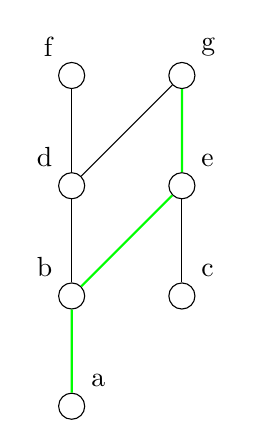
\begin{tikzpicture}[scale=.7]
  \node[circle, draw=black, text=black, label={135:f}] (f) at (0, 0) {};
  \node[circle, draw=black, text=black, label={45:g}] (g) at (2, 0) {};
  \node[circle, draw=black, text=black, label={135:d}] (d) at (0, -2) {};
  \node[circle, draw=black, text=black, label={45:e}] (e) at (2, -2) {};
  \node[circle, draw=black, text=black, label={135:b}] (b) at (0, -4) {};
  \node[circle, draw=black, text=black, label={45:c}] (c) at (2, -4) {};
  \node[circle, draw=black, text=black, label={45:a}] (a) at (0, -6) {};

  \draw [green, thick] (a) -- (b) -- (e) -- (g);
  \draw (b) -- (d) -- (f);
  \draw (c) -- (e);
  \draw (d) -- (g);
\end{tikzpicture}

% NOTE(ywen) >>>>>>>>>>>>>>>>>>>>>>>>>>>>>>>>>>>>>>>>>>>>>>>>>>
\noindent\rule[-9pt]{1cm}{10pt}\rule{10cm}{0.4pt}

\colorbox{lime}{NOTE(ywen)}: Why do we draw the diagram based on the covering relations?

Probably because drawing based on covering relations can produce the minimal diagram that still preserve all the binary
relations between elements. For example, in the ordered set $S = \{a, b, c\}$ where $a \leqslant b, b \leqslant c$. The
relation $a \leqslant c$ can be implied by the transitivity of ordered set, but it is not a covering relation.

If we only use the covering relations to draw diagrams, we only need to draw two segments for this set $S$:

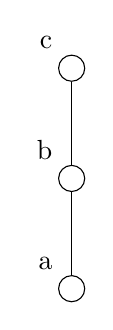
\begin{tikzpicture}[scale=.7]
  \node[circle, draw=black, text=black, label={135:a}] (a) at (0, 0) {};
  \node[circle, draw=black, text=black, label={135:b}] (b) at (0, 2) {};
  \node[circle, draw=black, text=black, label={135:c}] (c) at (0, 4) {};

  \draw (a) -- (b) -- (c);
\end{tikzpicture}

However, should we have been required to draw diagrams using all the relations, we'd have to draw three segments for
$S$, making the diagram more complicated:

\begin{tikzpicture}[scale=.7]
  \node[circle, draw=black, text=black, label={135:a}] (a) at (0, 0) {};
  \node[circle, draw=black, text=black, label={45:b}] (b) at (2, 2) {};
  \node[circle, draw=black, text=black, label={135:c}] (c) at (0, 4) {};

  \draw (a) -- (b) -- (c);
  \draw (a) -- (c);
\end{tikzpicture}

If $S$ is a very large set, drawing based on all relations can make the diagram messier. However, drawing based on the
covering relations can make the diagram more concise while still deliver all the needed ordering information.

\noindent\rule{10cm}{0.4pt}\rule{1cm}{10pt}
% <<<<<<<<<<<<<<<<<<<<<<<<<<<<<<<<<<<<<<<<<<<<<<<<<< NOTE(ywen)

% ------------------------------
\subsubsection{Lemma 1.17}
% ------------------------------

Let $P$ and $Q$ be finite ordered sets and let $\phi: P \rightarrow Q$ be a bijective function. Then the following are
equivalent:
\begin{enumerate}
  \item[(i)] $\phi$ is an order-isomorphism.
  \item[(ii)] $x < y$ in $P$ if and only if $\phi(x) < \phi(y)$ in $Q$.
  \item[(iii)] $x \lessdot y$ in $P$ if and only if $\phi(x) \lessdot \phi(y)$ in $Q$.
\end{enumerate}

% ------------------------------
\subsubsection{Proposition 1.18}
% ------------------------------

Two finite ordered sets $P$ and $Q$ are order-isomorphism if and only if they can be drawn with identical diagrams.

% =============================================================================
\section{Constructing/destructing ordered sets}
% =============================================================================

% ******************************
\subsection{Duality}
% ******************************

Given any ordered set $P$, we can form a new ordered set $P^{\theta}$ (the \textbf{dual} of P) by defining $x \leqslant y$
to hold in $P^{\theta}$ if and only if $y \leqslant x$ holds in $P$. For $P$ finite, we obtain a diagram for $P^{\theta}$
simply by \textbf{``turning upside down''} a diagram for P.

In general, given any statement $\Phi$ about ordered sets, we obtain the \textbf{dual statement} $\Phi^{\theta}$ by
replacing each occurrence of $\leqslant$ by $\geqslant$ and vice versa.

% ------------------------------
\subsubsection{The Duality Principle}
% ------------------------------

Given a statement $\Phi$ about ordered sets which is true in \textbf{all} ordered sets, the dual statement $\Phi^{\theta}$
is also true in \textbf{all} ordered sets.

% ******************************
\subsection{Bottom and top}
% ******************************

Let $P$ be an ordered set. We say $P$ has a bottom element if there exists $\bot \in P$ (called \textbf{bottom}) with
the property that $\forall x \in P. (\bot \leqslant x)$. Dually, $P$ has a top element if there exists $\top \in P$
such that $\forall x \in P. (x \leqslant \top)$ (called \textbf{top}).

Note that:
\begin{enumerate}
  \item $\bot$ is \textbf{unique} when it exists; dually, $\top$ is \textbf{unique} when it exists.
        \begin{itemize}
          \item The proof is simple: Suppose the bottom exists and there are two bottoms $b_1, b_2 \in P$ and $b_1 \ne b_2$.
                By definition of bottom, $b_1 \leqslant b_2$ and $b_2 \leqslant b_1$, but by definition of an ordered
                set, $(b_1 \leqslant b_2 \land b_2 \leqslant b_1) \rightarrow b_1 = b_2$, which contradicts with the
                assumption that $b_1 \ne b_2$. So if an ordered set $P$ has a bottom, it must be unique.
        \end{itemize}
  \item $\bot$ or $\top$ \textbf{may not always exist}, because the definition requires $\bot$ or $\top$ be comparable
        with \textbf{every other} element in $P$ but this may not always be true. As a result:
        \begin{itemize}
          \item A finite chain always has bottom and top elements.
          \item An infinite chain may not. For example, $\mathbb{N}$ has bottom element $1$ but no top; $\mathbb{Z}$
                has neither bottom nor top.
          \item Bottom and top do not exist in any antichains with more than one element.
        \end{itemize}
\end{enumerate}

% ------------------------------
\subsubsection{Lifting} \label{ch01-lifting}
% ------------------------------

Lack of a bottom element can be easily remedied by adding one. Given an ordered set $P$ (with or without $\bot$), we
form $P_{\bot}$ (called $P$ \textbf{``lifted''}) as follows. Take an element $\mathbf{0} \notin P$, define $P_{\bot} =
  P \cup \{\mathbf{0}\}$, and define $\leqslant$ by
\[x \leqslant y \leftrightarrow (\forall x, y \in P. (x = \mathbf{0} \lor x \leqslant y))\]

Intuitively, we just defined an element $\mathbf{0}$ that is less than every other element in $P$.

% ------------------------------
\subsubsection{Flat}
% ------------------------------

Any set $S$ can be transformed into a ordered set with $\bot$ as follows:
\begin{enumerate}
  \item[Step 1]: Order $S$ by making it an antichain $\bar{S}$.
  \item[Step 2]: Form $\bar{S}_{\bot}$ by following the steps in the section \ref{ch01-lifting}.
\end{enumerate}

The ordered set $\bar{S}_{\bot}$ that's obtained in this way is called a \textbf{flat}. Intuitively, all the elements
in $S$ are ``flattened'' and a bottom is added below all of them.

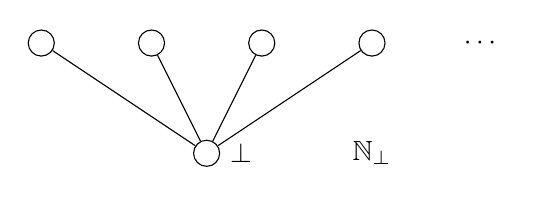
\begin{tikzpicture}[scale=.7]
  \node[circle, draw=black, text=black]                   (a) at (0, 0)  {};
  \node[circle, draw=black, text=black]                   (b) at (2, 0)  {};
  \node[circle, draw=black, text=black]                   (c) at (4, 0)  {};
  \node[circle, draw=black, text=black]                   (d) at (6, 0)  {};
  \node                                                   (e) at (8, 0)  {$\cdots$};
  \node[circle, draw=black, text=black, label={0:$\bot$}] (f) at (3, -2) {};
  \node                                                   (g) at (6, -2)  {$\mathbb{N}_{\bot}$};

  \draw (a) -- (f);
  \draw (b) -- (f);
  \draw (c) -- (f);
  \draw (d) -- (f);
\end{tikzpicture}

% ******************************
\subsection{Maximal/minimal/maximum/minimum}
% ******************************

Let $P$ be an ordered set and let $Q \subset P$. Then $a \in Q$ is a \textbf{maximal element} of $Q$ if $\forall x \in
  Q. (a \leqslant x \rightarrow a = x)$. There can be multiple maximal elements in $Q$. We denote the set of maximal
elements of $Q$ by \textbf{Max$Q$}. If $Q$ has a top element $\top_{Q}$, then Max$Q$ = \{$\top_{Q}$\}. In this case,
$\top_{Q}$ is called the \textbf{greatest} (or \textbf{maximum}) element of $Q$. We write $\top_{Q}$ = max$Q$.

A \textbf{minimal element}, the \textbf{least} (or \textbf{minimum}) element of $Q$, if they exist, are defined dually.

% NOTE(ywen) >>>>>>>>>>>>>>>>>>>>>>>>>>>>>>>>>>>>>>>>>>>>>>>>>>
\noindent\rule[-9pt]{1cm}{10pt}\rule{10cm}{0.4pt}

\colorbox{lime}{NOTE(ywen)}: Understanding the definition of ``maximal element''.

Note that, $\forall m, n \in Q$, they can have one of the following relations, by definition of ordered sets:
\begin{enumerate}
  \item $m \leqslant n \land m \ngeqslant n$
  \item $m \geqslant n \land m \nleqslant n$
  \item $m = n$ (i.e., $m \leqslant n \land m \geqslant n$)
  \item $m \parallel n$ (i.e., $m \nleqslant n \land m \ngeqslant n$)
\end{enumerate}

The definition of maximal element of $Q$ needs to compare $a$ with \textbf{every other} element $x$ in $Q$. So, of
course, there can be four theoretically possible results:
\begin{enumerate}
  \item $a \leqslant x \land a \ngeqslant x$
  \item $a \geqslant x \land a \nleqslant x$
  \item $a = x$ (i.e., $a \leqslant x \land a \geqslant x$)
  \item $a \parallel x$ (i.e., $a \nleqslant x \land a \ngeqslant x$)
\end{enumerate}

Observe that $a \leqslant x$ occurs in case 1 and case 3. The definition then says $\forall x \in Q. (a \leqslant x \rightarrow a = x)$.
This actually eliminates case 1 because $a \neq x$ in case 1. As a result, in $Q$, the element $a$, when compared to
any other element $x$, is either greater than $x$ (i.e., case 2), or equal to $x$ (i.e., case 3), or not comparable
(i.e., case 4). But $a$ is \textbf{never} less than $x$. We thus call $a$ a \textbf{maximal} element.

\colorbox{lime}{NOTE(ywen)}: Therefore, in an antichain $S$, Max$S$ = Min$S$ = S (i.e., in an antichain, every element
is the maximal or the minimal element of the set that consists of only itself.)

\colorbox{lime}{NOTE(ywen)}: According to the definition of ``top'', the maximum must be comparable with every other
element in $Q$, while a maximal element may not be comparable with every other element in $Q$.

\noindent\rule{10cm}{0.4pt}\rule{1cm}{10pt}
% <<<<<<<<<<<<<<<<<<<<<<<<<<<<<<<<<<<<<<<<<<<<<<<<<< NOTE(ywen)

In general, a subset $Q$ of an ordered set $P$ may have many maximal elements, just one, or none. Note $P$ and its
subset $Q$ may be finite or infinite. Therefore, there are three cases to consider:

\begin{table}[H]
  \centering
  \begin{tabular}{|c|c|c|}
    \cline{1-3}
        & P        & $Q \subset P$ \\ [1ex] \cline{1-3}
    (1) & infinite & infinite      \\ [0.5ex] \cline{1-3}
    (2) & infinite & finite        \\ [0.5ex] \cline{1-3}
    (3) & finite   & finite        \\ [0.5ex] \cline{1-3}
  \end{tabular}
\end{table}

Intuitively, the number of maximal elements in $Q$ depends on whether $Q$ is ``bounded above'' (see real mathematical
analysis). If $Q$ is bounded above, it has maximal elements; if $Q$ is not bounded above, it doesn't have any maximal
elements. For example:
\begin{enumerate}
  \item[(1)] Consider $P = \mathbb{N}$ which is an infinite ordered set:
        \begin{enumerate}
          \item Its subset $Q = \{x: x = 2n, n \in \mathbb{N}\}$ does not have any maximal elements because $Q$ is not
                ``bounded above''.
          \item Its subset $Q = \{x: x \leqslant 0, n \in \mathbb{N}\}$ has one maximal element (which is also its
                maximum) 0.
        \end{enumerate}
  \item [(1')] (Still consider case (1)) Consider $P = \mathcal{P}(\mathbb{N})$ which is an infinite ordered set:
        \begin{enumerate}
          \item $\mathbb{N}$ is the only top element in $P$ (In contrast, $\emptyset$ is the only bottom element in
                $P$). Therefore, its subset $Q = P \setminus \mathbb{N}$ does not have any top element. However,
                $\forall n \in \mathbb{N}, \mathbb{N} \setminus \{n\} \in MaxQ$. Intuitively, in the Hasse diagram of
                $\mathcal{P}(\mathbb{N})$, $\mathbb{N}$ is the only element on the top level (hence the top element).
                Immediately below it are all the subsets of $\mathbb{N} \setminus \{n\}$ which are the maximal elements
                in $\mathcal{P}(\mathbb{N}) \setminus \mathbb{N}$.
          \item Its subset $Q$ that consists of all \textbf{finite} subsets of $\mathbb{N}$ does not have any maximal
                elements. Consider a finite subset of $\mathbb{N}$: $\{1, 2, \ldots, k\}, k \in \mathbb{N}$. It's true
                that this subset is either greater than the subsets ``immediately below'' it (e.g., $\emptyset$,
                $\{1, 2, \ldots, k-1\}$, $\{1, 2, \ldots, k-2\}$) or is not comparable with other finite subsets (e.g.,
                $\{k+1, k+2, \ldots, k+m\}$). Therefore, it looks like $\{1, 2, \ldots, k\}$ could be a maximal element.
                However, there is always another finite subset of $\mathbb{N}$, $\{1, 2, \ldots, k, k+1\}$, that is
                greater than $\{1, 2, \ldots, k\}$. Therefore, there is no ``upper bound'', hence no maximal elements.
        \end{enumerate}
  \item[(2)] It's easy to see that a finite nonempty subset $Q$ has at least one maximal element; if $Q$ is $\emptyset$,
        it doesn't have any maximal element.
  \item[(3)] It's easy to see that a finite nonempty subset $Q$ has at least one maximal element; if $Q$ is $\emptyset$,
        it doesn't have any maximal element.
\end{enumerate}

% ******************************
\subsection{Sums of ordered sets}
% ******************************

The ordered sets $P$ and $Q$ we consider here are \textbf{disjoint}. This is no real restriction since we can always
find isomorphic copies of the original ordered sets which are disjoint; see Exercise 1.9 for a. formal approach to this
process.

% ------------------------------
\subsubsection{Disjoint union}
% ------------------------------

Suppose that $P$ and $Q$ are (disjoint) ordered sets. The \textbf{disjoint union} $P \dot{\cup} Q$ of $P$ and $Q$ is
the ordered set formed by defining $x \leqslant y$ in $P \dot{\cup} Q$ if and only if either ($x,y \in P$ and
$x \leqslant y$ in P) or ($x,y \in Q$ and $x \leqslant y$ in Q).

A diagram for $P \dot{\cup} Q$ is formed by placing \textbf{side by side} diagrams for $P$ and $Q$.

% ------------------------------
\subsubsection{Linear sum}
% ------------------------------

Suppose that $P$ and $Q$ are (disjoint) ordered sets. The \textbf{linear sum} $P \oplus Q$ is defined by taking the
following order relation on $P \cup Q: x \leqslant y$ if and only if:
\begin{align*}
        & x, y \in P \land x \leqslant y, \\
  or \  & x, y \in Q \land x \leqslant y, \\
  or \  & x \in P \lor y \in Q
\end{align*}

A diagram for $P \oplus Q$ (when $P$ and $Q$ are finite) is obtained by placing a diagram for $P$ directly below a
diagram for $Q$ and then adding a line segment from each maximal element of $P$ to each minimal element of $Q$.

% ------------------------------
\subsubsection{Associativity}
% ------------------------------

The operations $\dot{\cup}$ and $\oplus$ are both associative: for pairwise disjoint ordered sets $P$, $Q$, and $R$:
\[P \dot{\cup} (Q \dot{\cup} R) = (P \dot{\cup} Q) \dot{\cup} R\]
and
\[P \oplus (Q \oplus R) = (P \oplus Q) \oplus R\]

% ------------------------------
\subsubsection{$\mathbf{M}_n$}
% ------------------------------

We denote by $\mathbf{M}_n$ the linear sum $\mathbf{1} \oplus \bar{\mathbf{n}} \oplus \mathbf{1}$.

% ******************************
\subsection{Products} \label{ch01-products}
% ******************************

Let $P_1, \ldots, P_n$ be ordered sets. The Cartesian product $P_1 \times \cdots \times P_n$ can be made into an ordered
set by imposing the coordinate-wise order defined by:
\[
  (x_1, \ldots, x_n) \leqslant (y_1, \ldots, y_n) \Leftrightarrow (\forall i) x_i \leqslant y_i \ in \ P_i
\]

Given an ordered set $P$, the notation $P^n$ is used as shorthand for the n-fold product $P \times \ldots \times P$.

% NOTE(ywen) >>>>>>>>>>>>>>>>>>>>>>>>>>>>>>>>>>>>>>>>>>>>>>>>>>
\noindent\rule[-9pt]{1cm}{10pt}\rule{10cm}{0.4pt}

\colorbox{lime}{NOTE(ywen)}: More on the Cartesian product.

In general, given two sets $A$ and $B$, its Cartesian product $A \times B$ is defined as $\{(a, b) | a \in A \land b \in B\}$.
Therefore, suppose $A = \{x, y\}$ and $B = \{1, 2\}$, then $A \times B = \{(x, 1), (x, 2), (y, 1), (y, 2)\}$.

This can be applied to any $n$ sets: Given sets $P_1, \ldots, P_n$, the Cartesian product $P_1 \times \cdots \times P_n$
is defined as $\{(p_1, \ldots, p_n) | p_1 \in P_1 \land \ldots \land p_n \in P_n\}$. Here, $p_i$ can be seen as an
arbitrarily chosen element from the set $P_i$.

If $P_1$ is an ordered set, that means given any two elements from $P_i$, denoted as $p_{11}$ and $p_{12}$, we have
$p_{11} \leqslant p_{12}$ or $p_{12} \leqslant p_{11}$. Let's just assume it's $p_{11} \leqslant p_{12}$. This can be
applied to $P_2, \ldots, P_n$, namely, we can have $p_{21} \leqslant p_{22}$, $\ldots$, $p_{n1} \leqslant p_{n2}$.

Then both $(p_{11}, p_{21}, \ldots, p_{n1})$ and $(p_{12}, p_{22}, \ldots, p_{n2})$ are elements of the Cartesian
product $P_1 \times \cdots \times P_n$. If we use $x_i$ to denote $p_{1i}$, and use $y_i$ to denote $p_{2i}$, then we
have $(x_1, \ldots, x_n)$ and $(y_1, \ldots, y_n)$ are both elements in $P_1 \times \cdots \times P_n$.

\colorbox{lime}{NOTE(ywen)}: Not all the elements in $P_1 \times \cdots \times P_n$ are comparable.

Note that the order that's defined on the Cartesian product $P_1 \times \cdots \times P_n$ requires that \textbf{every}
pair of $x_i$ and $y_i$ must be $x_i \leqslant y_i$. Therefore, for two elements $(x_1, \ldots, x_n)$ and $(y_1, \ldots, y_n)$,
if $x_1 \leqslant y_1$, $\ldots$, $x_{k-1} \leqslant y_{k-1}$, $x_{k+1} \leqslant y_{k+1}$, $\ldots$, $x_n \leqslant y_n$,
but $x_k > y_k$, then $(x_1, \ldots, x_n)$ and $(y_1, \ldots, y_n)$ are \textbf{not} comparable.

\noindent\rule{10cm}{0.4pt}\rule{1cm}{10pt}
% <<<<<<<<<<<<<<<<<<<<<<<<<<<<<<<<<<<<<<<<<<<<<<<<<< NOTE(ywen)

% ------------------------------
\subsubsection{Hasse diagrams for products (example 1)}
% ------------------------------

Consider the two ordered sets:
\begin{enumerate}
  \item $P = \{1, 2\}$ where $1, 2 \in \mathbb{N}$, so $1 \lessdot 2$.
  \item $Q = \{7, 8, 9\}$ where $7, 8, 9 \in \mathbb{N}$, so $7 \lessdot 8 \lessdot 9$.
\end{enumerate}

So the Hasse diagrams for $P$ and $Q$ are:

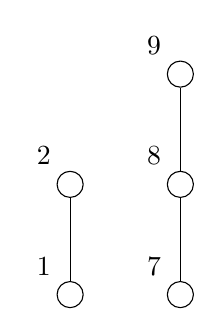
\begin{tikzpicture}[scale=.7]
  \node[circle, draw=black, text=black, label={135:1}] (1) at (0, 0) {};
  \node[circle, draw=black, text=black, label={135:2}] (2) at (0, 2) {};

  \node[circle, draw=black, text=black, label={135:7}] (7) at (2, 0) {};
  \node[circle, draw=black, text=black, label={135:8}] (8) at (2, 2) {};
  \node[circle, draw=black, text=black, label={135:9}] (9) at (2, 4) {};

  \draw (1) -- (2);
  \draw (7) -- (8) -- (9);
\end{tikzpicture}

The product of $P \times Q = \{(1, 7), (1, 8), (1, 9), (2, 7), (2, 8), (2, 9)\}$. According to the order defined above
for the product, we have:
\begin{enumerate}
  \item $(1, 7) \leqslant (1, 8) \leqslant (1, 9)$
  \item $(2, 7) \leqslant (2, 8) \leqslant (2, 9)$
  \item $(1, 7) \leqslant (2, 7)$
  \item $(1, 8) \leqslant (2, 8)$
  \item $(1, 9) \leqslant (2, 9)$
  \item $(1, 8)$ and $(2, 7)$ are not comparable.
  \item $(1, 9)$ and $(2, 7)$ are not comparable.
  \item $(1, 9)$ and $(2, 8)$ are not comparable.
\end{enumerate}

We can also see the covering relations as follows:
\begin{enumerate}
  \item $(1, 7) \lessdot (1, 8) \lessdot (1, 9)$
  \item $(2, 7) \lessdot (2, 8) \lessdot (2, 9)$
  \item $(1, 7) \lessdot (2, 7)$
  \item $(1, 8) \lessdot (2, 8)$
  \item $(1, 9) \lessdot (2, 9)$
\end{enumerate}

So we can draw the following Hasse diagram for $P \times Q$:

\begin{tikzpicture}[scale=.7]
  \node[circle, draw=black, text=black, label={-45:(1, 7)}] (17) at (0, 0) {};
  \node[circle, draw=black, text=black, label={-45:(1, 8)}] (18) at (2, 2) {};
  \node[circle, draw=black, text=black, label={-45:(1, 9)}] (19) at (4, 4) {};
  \node[circle, draw=black, text=black, label={135:(2, 7)}] (27) at (-2, 2) {};
  \node[circle, draw=black, text=black, label={135:(2, 8)}] (28) at (0, 4) {};
  \node[circle, draw=black, text=black, label={135:(2, 9)}] (29) at (2, 6) {};

  \draw (17) -- (18) -- (19);
  \draw (27) -- (28) -- (29);
  \draw (17) -- (27);
  \draw (18) -- (28);
  \draw (19) -- (29);
\end{tikzpicture}

Note that $(1, 8)$ and $(2, 7)$ are not connected because they are not comparable; $(1, 9)$ and $(2, 7)$ are not
connected because they are not comparable; $(1, 9)$ and $(2, 8)$ are not connected because they are not comparable.

% ------------------------------
\subsubsection{Hasse diagrams for products (example 2)}
% ------------------------------

Let's consider $\mathbf{2}^4 = \mathbf{2} \times \mathbf{2} \times \mathbf{2} \times \mathbf{2}$, where
$\mathbf{2} = \{0, 1\}$ (according to \ref{ch01-chains-and-antichains}). The elements in $\mathbf{2}^4$ are:
\begin{enumerate}
  \item $(0, 0, 0, 0)$
  \item $(0, 0, 0, 1)$
  \item $(0, 0, 1, 0)$
  \item $(0, 0, 1, 1)$
  \item $(0, 1, 0, 0)$
  \item $(0, 1, 0, 1)$
  \item $(0, 1, 1, 0)$
  \item $(0, 1, 1, 1)$
  \item $(1, 0, 0, 0)$
  \item $(1, 0, 0, 1)$
  \item $(1, 0, 1, 0)$
  \item $(1, 0, 1, 1)$
  \item $(1, 1, 0, 0)$
  \item $(1, 1, 0, 1)$
  \item $(1, 1, 1, 0)$
  \item $(1, 1, 1, 1)$
\end{enumerate}

To study the order (which is defined in \ref{ch01-products}) of these elements, we can group them according to how many
1's there are in each element:
\begin{itemize}
  \item Zero 1: $(0, 0, 0, 0)$
  \item One 1: $(0, 0, 0, 1)$, $(0, 0, 1, 0)$, $(0, 1, 0, 0)$, $(1, 0, 0, 0)$
  \item Two 1's: $(0, 0, 1, 1)$, $(0, 1, 0, 1)$, $(1, 0, 0, 1)$, $(0, 1, 1, 0)$, $(1, 0, 1, 0)$, $(1, 1, 0, 0)$
  \item Three 1's: $(0, 1, 1, 1)$, $(1, 0, 1, 1)$, $(1, 1, 0, 1)$, $(1, 1, 1, 0)$
  \item Four 1's: $(1, 1, 1, 1)$
\end{itemize}

So we can draw the following Hasse diagram for $\mathbf{2}^4$:

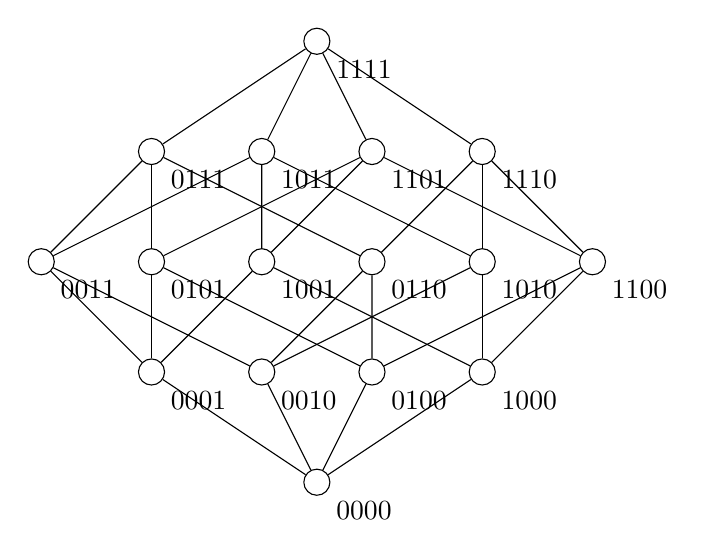
\begin{tikzpicture}[scale=.7]
  \node[circle, draw=black, text=black, label={-45:0000}] (0000) at (5, 0) {};
  \node[circle, draw=black, text=black, label={-45:0001}] (0001) at (2, 2) {};
  \node[circle, draw=black, text=black, label={-45:0010}] (0010) at (4, 2) {};
  \node[circle, draw=black, text=black, label={-45:0100}] (0100) at (6, 2) {};
  \node[circle, draw=black, text=black, label={-45:1000}] (1000) at (8, 2) {};
  \node[circle, draw=black, text=black, label={-45:0011}] (0011) at (0, 4) {};
  \node[circle, draw=black, text=black, label={-45:0101}] (0101) at (2, 4) {};
  \node[circle, draw=black, text=black, label={-45:1001}] (1001) at (4, 4) {};
  \node[circle, draw=black, text=black, label={-45:0110}] (0110) at (6, 4) {};
  \node[circle, draw=black, text=black, label={-45:1010}] (1010) at (8, 4) {};
  \node[circle, draw=black, text=black, label={-45:1100}] (1100) at (10, 4) {};
  \node[circle, draw=black, text=black, label={-45:0111}] (0111) at (2, 6) {};
  \node[circle, draw=black, text=black, label={-45:1011}] (1011) at (4, 6) {};
  \node[circle, draw=black, text=black, label={-45:1101}] (1101) at (6, 6) {};
  \node[circle, draw=black, text=black, label={-45:1110}] (1110) at (8, 6) {};
  \node[circle, draw=black, text=black, label={-45:1111}] (1111) at (5, 8) {};

  \draw (0000) -- (0001);
  \draw (0000) -- (0010);
  \draw (0000) -- (0100);
  \draw (0000) -- (1000);
  \draw (0001) -- (0011);
  \draw (0001) -- (0101);
  \draw (0001) -- (1001);
  \draw (0010) -- (0011);
  \draw (0010) -- (0110);
  \draw (0010) -- (1010);
  \draw (0100) -- (0101);
  \draw (0100) -- (0110);
  \draw (0100) -- (1100);
  \draw (1000) -- (1001);
  \draw (1000) -- (1010);
  \draw (1000) -- (1100);
  \draw (0011) -- (0111);
  \draw (0011) -- (1011);
  \draw (0101) -- (0111);
  \draw (0101) -- (1101);
  \draw (1001) -- (1011);
  \draw (1001) -- (1101);
  \draw (0110) -- (0111);
  \draw (0110) -- (1110);
  \draw (1010) -- (1011);
  \draw (1010) -- (1110);
  \draw (1100) -- (1101);
  \draw (1100) -- (1110);
  \draw (0111) -- (1111);
  \draw (1011) -- (1111);
  \draw (1101) -- (1111);
  \draw (1110) -- (1111);
\end{tikzpicture}

% ------------------------------
\subsubsection{Lexicographic order}
% ------------------------------

Consider the ordered sets $X$ and $Y$. If we use the ordered defined above, then not all the elements in the product
$X \times Y$ are comparable (see my notes above). However, we can also define the \textbf{lexicographic order}:
\[
  (x_1, x_2) \leqslant (y_1, y_2) \Leftrightarrow ((x_1 < y_1) \lor (x_1 = y_1 \land x_2 \leqslant y_2))
\]

By iteration a lexicographic order can be defined on any \textbf{finite} product of ordered sets.
\colorbox{red}{TODO(ywen):} Can lexicographic order be defined on finite product of ordered sets only?

% ******************************
\subsection{Proposition}
% ******************************

Let $X = \{1, 2, \ldots, n\}$ and define $\phi: \mathcal{P}(X) \rightarrow \mathbf{2}^n$ by $\phi(A) = (\epsilon_1, \ldots, \epsilon_n)$
where
\[
  \epsilon_i = \begin{cases}
    1, & if \ i \in A    \\
    0, & if \ i \notin A
  \end{cases}
\]

Then $\phi$ is an order-isomorphism.

% NOTE(ywen) >>>>>>>>>>>>>>>>>>>>>>>>>>>>>>>>>>>>>>>>>>>>>>>>>>
\noindent\rule[-9pt]{1cm}{10pt}\rule{10cm}{0.4pt}

\colorbox{lime}{NOTE(ywen)}: Understanding the proposition: Before we look at its proof, we need to understand what
this proposition is talking about. We can use $n = 2$ to understand it. When $n = 2$, the left side of $\phi$ is:
\[
  \{\emptyset, \{1\}, \{2\}, \{1, 2\}\}
\]

The right side of $\phi$ is
\[
  \mathbf{2}^2 = \{0, 1\} \times \{0, 1\} = \{(0, 0), (0, 1), (1, 0), (1, 1)\}
\]

So $\phi$ maps every element in $\mathcal{P}(\{1, 2\})$ to an element in $\{(0, 0), (0, 1), (1, 0), (1, 1)\}$ with the
following rules:
\begin{enumerate}
  \item Let $\phi(\emptyset) = (\epsilon_1, \epsilon_2)$. Because $1 \notin \emptyset$, $\epsilon_1 = 0$; because
        $2 \notin \emptyset$, $\epsilon_2 = 0$. Therefore, $\phi(\emptyset) = (0, 0)$.
  \item Let $\phi(\{1\}) = (\epsilon_1, \epsilon_2)$. Because $1 \in \{1\}$, $\epsilon_1 = 1$; because $2 \notin \{1\}$,
        $\epsilon_2 = 0$. Therefore, $\phi(\{1\}) = (1, 0)$.
  \item Let $\phi(\{2\}) = (\epsilon_1, \epsilon_2)$. Because $1 \notin \{2\}$, $\epsilon_1 = 0$; because $2 \in \{2\}$,
        $\epsilon_2 = 1$. Therefore, $\phi(\{2\}) = (0, 1)$.
  \item Let $\phi(\{1, 2\}) = (\epsilon_1, \epsilon_2)$. Because $1 \in \{1, 2\}$, $\epsilon_1 = 1$; because $2 \in \{1, 2\}$,
        $\epsilon_2 = 1$. Therefore, $\phi(\{1, 2\}) = (1, 1)$.
\end{enumerate}

The proposition is trying to say that $\phi$ is an order-isomorphism.

\noindent\rule{10cm}{0.4pt}\rule{1cm}{10pt}
% <<<<<<<<<<<<<<<<<<<<<<<<<<<<<<<<<<<<<<<<<<<<<<<<<< NOTE(ywen)

\colorbox{red}{TODO(ywen):} Study the proof.

\colorbox{red}{TODO(ywen):} On 2024-02-15, I decided to stop here. I started to learn the order theory in order to
understand the differences between maximal/minimal and maximum/minimum, but obviously I have gone way further than
originally planned. I will resume the learning of this textbook if needed.

% =============================================================================
%
% References
%
% =============================================================================

\chapter*{References}
\addcontentsline{toc}{chapter}{References}

\begin{itemize}
  \item $[1]$ \href{https://www.cambridge.org/core/books/introduction-to-lattices-and-order/946458CB6638AF86D85BA00F5787F4F4}{B. A. Davey, H. A. Priestley: \it{Introduction to Lattices and Order}}
\end{itemize}

\end{document}
